\documentclass[USenglish,oneside,twocolumn]{article}
\usepackage{color}
\usepackage[hyphens]{url}
\usepackage{longtable}
\usepackage{graphicx}
\usepackage{enumitem}
\usepackage{pdfpages}
\usepackage{adjustbox}
%\usepackage{hyperref}

\usepackage[utf8]{inputenc}%(only for the pdftex engine)
%\RequirePackage[no-math]{fontspec}%(only for the luatex or the xetex engine)
\usepackage[big]{dgruyter_NEW}
 
\hyphenation{Isa-bela}

\DOI{foobar}

\cclogo{
\includegraphics{by-nc-nd.pdf}}

% Format a participant quotation.
\newcommand{\pquote}[2]{
\begin{quotation}
\noindent #1:~\textit{``#2''}
\end{quotation}
}
  
\begin{document}
   \author*[1]{Author 1}

  \author[2]{Author 2}

  \author[3]{Author 3}

  \author[4]{Author 4}

  \author[5]{Author 5}
  
  \author[6]{Author 6}

  \affil[1]{Affiliation of Author 1, E-mail: \mbox{author1@affiliation.edu}}
  \affil[2]{Affiliation of Author 2, E-mail: \mbox{author2@affiliation.edu}}
  \affil[3]{Affiliation of Author 3, E-mail: \mbox{author3@affiliation.edu}}
  \affil[4]{Affiliation of Author 4, E-mail: \mbox{author4@affiliation.edu}}
  \affil[5]{Affiliation of Author 5, E-mail: \mbox{author5@affiliation.edu}}
  \affil[6]{Affiliation of Author 6, E-mail: \mbox{author6@affiliation.edu}}
%  \author*[1]{Linda Lee}
%
%  \author[2]{David Fifield}
%
%  \author[3]{Nathan Malkin}
%
%  \author[4]{Ganesh Iyer}
%
%  \author[5]{Serge Egelman}
%  
%  \author[6]{David Wagner}
%
%  \affil[1]{University of California Berkeley, E-mail: \mbox{lnl@cs.berkeley.edu}}
%
%  \affil[2]{University of California Berkeley, E-mail: \mbox{fifield@cs.berkeley.edu}}
%
%  \affil[3]{University of California Berkeley, E-mail: \mbox{nmalkin@cs.berkeley.edu}}
%
%  \affil[4]{University of California Berkeley, E-mail: \mbox{ganesh.v@berkeley.edu}}
%  
%  \affil[5]{University of California Berkeley and International Computer Science Institute, E-mail: \mbox{egelman@cs.berkeley.edu}}
%   
%  \affil[6]{University of California Berkeley, E-mail: \mbox{daw@cs.berkeley.edu}}

  \title{\huge A Better (One-Line!) Title Here}

  \runningtitle{A Better (One-Line!) Title Here}

  %\subtitle{...}

  \begin{abstract}
{
We evaluate, design, and test the Tor Launcher interface by
placing users in simulated censorship environments, instructing them to use Tor
to circumvent censorship, and measuring their interface interactions.
A 16-participant qualitative study examines user assumptions and common mistakes.
We use the results as feedback to redesign the configuration interface.
A 114-participant quantitative study shows that our design changes result in
a significant reduction in time. We conclude with recommendations for changes 
to the current interface as well as alternative solutions.}
\end{abstract}
  \keywords{Usable Security, User Studies, Tor, Security, Censorship, Anonymity}
%  \classification[PACS]{}
 % \communicated{...}
 % \dedication{...}

  \journalname{Proceedings on Privacy Enhancing Technologies}
\DOI{Editor to enter DOI}
  \startpage{1}
  \received{..}
  \revised{..}
  \accepted{..}

  \journalyear{2015}
  \journalvolume{2015}
  \journalissue{2}

\maketitle

\section{Introduction}

Tor~\cite{dingledine2004tor} is an anonymity network that routes Internet traffic through a series of relays 
that make it difficult to observe the source and destination. 
Tor Browser~\cite{torbrowser} is a modified Firefox browser with a built-in Tor client that
is the recommended way to use Tor. Tor Launcher is a Tor Browser component that
starts, stops, and otherwise controls the underlying Tor processes.
Tor Launcher's graphical user interface asks the user to configure
bridges, pluggable transports, and proxies to make a connection to Tor (we refer to this graphical user interface as the ``configuration interface'' throughout this paper). This is the object of our study. 

We hope that our work helps users more easily connect to Tor. The direct and obvious benefit of our work is that is that it may help users who would have previously been unable to configure Tor Browser to use it or that it may save time for users who would have been able to configure a valid connection to the Tor. Improving the user experience through user testing has the potential to be beneficial for both the software company (less help desk tickets) and the end users (less frustration). 

However, we believe that our work uniquely necesssary and beneficial to Tor Browser. Although originally designed for Internet anonymity, using Tor Browser to circumvent censorship has now become sufficiently common that many countries now attempt to block Tor relays for this reason~\cite{winter2012great}. Our contributions toward an easier bootstrapping process will especially benefit citizens who face Internet censorship. If there is an increase in overall users as a result, they add a security bonus by increasing the anonymity set~\cite{dingledine2006anonymity}. \\


\noindent This paper contributes:
\smallskip
\begin{itemize}
\item an evaluation of the current configuration interface
\item a redesigned configuration interface
\item logs of 114 users' connection attempts
\item failure modes seen during connection attempts
\item recommended interface changes
\item alternative bootstrapping approaches
\end{itemize}

We start by introducing relevant concepts (section~\ref{sec:background}) and
defining the scope of our experiment (section~\ref{sec:scope}). 
Then, we report user observations and interviews (section~\ref{sec:qualitative}),
list design principles and interface changes (section~\ref{redesign}),
state evaluation criteria for testing the interface (section~\ref{sec:eval}), 
and measure the impact of our design changes (Section~\ref{sec:quantitative}).
We end with a discussion on what we learned (section~\ref{sec:discussion}),
limitations of out experiment (section~\ref{sec:limitations}), 
a look at our work in the context of existing work (section~\ref{sec:related}), and
a brief conclusion (section~\ref{sec:conclusion}).

\section{Background}
\label{sec:background}
This section talks about network components involved in connecting to Tor, network conditions that require these network components, and examples of what users must currently do to connect to Tor. 

\subsection{Relays, Bridges, Pluggable Transports, and Proxies} 

Tor relays are routers in the Tor Network that receive and pass along Tor traffic. 
There are three types of Tor relays: guard relays that serve as an entry node, middle relays that forward traffic from an entry node to an exit node, and exit relays which directs traffic to the destination. 
Censors can block access to the Tor network by blocking these relays, which are publicly listed. 

Bridges are unlisted Tor relays that can serve as an alternative entry node.
Bridges can be simple, unlisted relays. 
But most bridges run a pluggable tranport (referred to as ``transport'' for shorthand) that obfuscates the traffic. 
Most transports disguise traffic to defeat on-the-wire identification, relying on the secrecy of their static IP addresses for their effectiveness.
These include ``fte'' and ``fte-ipv6''~\cite{fte},
which disguise the Tor protocol as another protocol (such as HTTP), and
``obfs3''~\cite{obfs3}, ``obfs4''~\cite{obfs4}, and ``scramblesuit''~\cite{scramblesuit},
which encrypt or alter the Tor protocol to appear as random noise.
Some transports route traffic through other services, avoiding the need for a secret IP address. 
``flashproxy''~\cite{flashproxy} connects through third parties' web browsers,
and the ``meek''~\cite{fifield2015blocking} options route traffic
through content delivery networks.
Bridges and transports allow a connection to the Tor network when all publicly listed relays and any Tor-looking packets are blocked. Fig.~\ref{fig:bridge-options} shows the bridge and transport options at the time of the study.

\begin{figure}
  \centering
    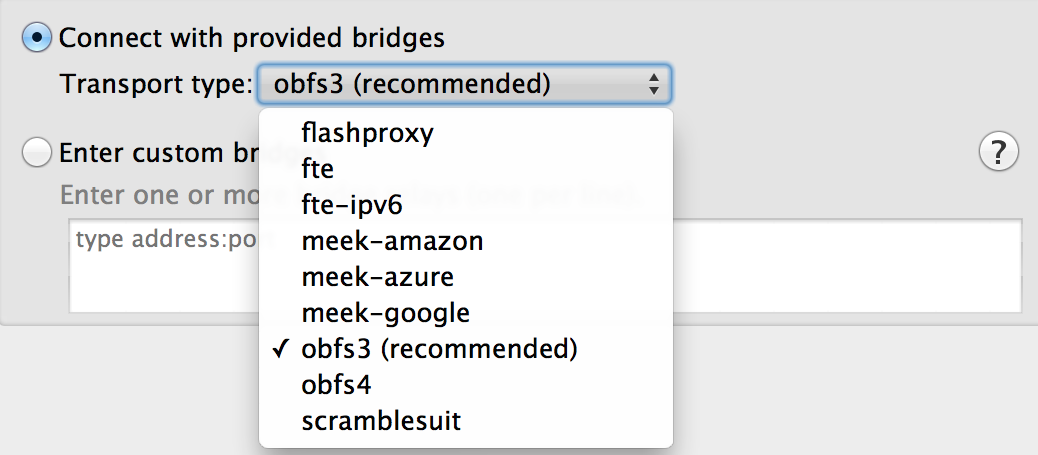
\includegraphics[width=0.5\textwidth]{bridge-options.png}
\caption{
Bridge options in Tor Browser~5.0.3's Tor Launcher interface.
Pre-configured bridges can be selected by ``Transport type,'' which refer to various
censorship circumvention technologies (``pluggable transports'').
%Under ``Enter custom bridges,'' there is a space to paste in
%a bridge line, obtained out of band.
%The ``Help'' button displays instructions on obtaining
%bridge lines. 
}
\label{fig:bridge-options}
\end{figure}

In addition to Tor-specific components, a local proxy is required to connect 
in certain managed networks. In this paper, ``proxy'' refers to a local, ordinary unobfuscated proxy such as a SOCKS or HTTP proxy. (Technically, Tor relays, bridges, and local proxies all allow indirect network connections to other network services and can be considered a proxy.) Fig.~\ref{fig:topology} illustrates the interacting components.

\begin{figure}
\centering

\includegraphics{topology.pdf}
\caption{
The chain of components involved in connecting to a website over Tor.
Most users do not need a proxy;
only users who face a censor need a bridge.
In the diagram, ``Tor'' represents all three anonymizing hops through the Tor network.
We have shown the bridge as a separate component
because of the special role it plays.
When a bridge is used, it becomes the first Tor relay.
}
\label{fig:topology}
\end{figure}

\subsection{State and Corporate Censorship}
State level censors can vary in their thoroughness in censorship, resulting in a variety of ever-changing network conditions. Some block websites with a combination of IP blacklisting and DNS-poisoning while others that employ more sophisticated techniques such as deep packet inspection and protocol detection. In countries that censor services but do not block censorship circumvention tools, any connection to Tor will byass the censorship. In other countries, sophisticated state-level censorship require bridges that run specific tranports that route traffic through other, non-Tor services first. For example, only meek-amazon and meek-azure transports work to bypass China's GFW. 

Some companies and educational institutions have a firewall, which can be bypassed with a proxy (with or without a connection to Tor). 

\subsection{Connecting to Tor} 
 
%\begin{itemize}
%	\item{Whether their Internet connection is censored} 
%	\item{Whether the Tor network is censored by their ISP}
%	\item{Which hard-coded bridges work in their country} 
%	\item{If no hard-coded bridges work, how to get a custom bridge and connect to it} 
%	\item{Whether a proxy is required to access the Internet}
%	\item{If a proxy is required, and if so, the proxy settings}
%\end{itemize}

Configuring a bridge requires providing one or more
``bridge lines,'' a specifically formatted bridge specification that
includes its IP address, transport type, and other metadata.
The interface has hard-coded options (see Figure~\ref{fig:bridge-options}) 
that select a group of bridges that use a particular transport.
For instance, choosing the hard-coded obfs3 option
configures a handful of bridges that use obfs3 transport.
If the built-in bridges do not work, a user can obtain bridge lines
through out-of-band channels, for instance by email~\cite{bridgedb}.

Configuring a proxy requires providing the proxy protocol, IP address, port, and additional optional fields. The user must locate and input this information. 

There are many valid configuration settings to connect to the Tor network.
For instance, a user who needs a bridge but not need a proxy can connect to Tor with a bridge and proxy, provided that both were configured correctly. The set of valid configuration settings vary on the specific network environment. 

\section{Methodology} 

\subsection{Testing Procedure} 
{\color {blue}

Procedure: inspection, formative, design, summative. 

We wanted to inspect the thing ourselves before doing formative testing so we know what to look for. 
http://www.usabilitybok.org/heuristic-walkthrough, not a pluralistic walkthrough (http://www.usabilitybok.org/pluralistic-walkthrough) or cognitive walkthrough (http://www.usabilitybok.org/cognitive-walkthrough). 

Most usability testing involves finding and fixing problems as part of an iterative design process to make an interface more usable. It is typically called a Formative Usability Evaluation. In contrast, a Summative Usability Evaluation describes the current usability of an interface—as measured by things like task times, completion rates and satisfaction scores. Summative tells you how usable an interface is and formative tells you what isn't usable.

Formative usability testing takes the role of a support tool for decision making during the beginning stages of the design process and - if applied early in the development process - provides valuable insights of where users have difficulty reaching their user goals with the technology (website, desktop GUI design, hardware product) or service.
%http://www.usabilitybok.org/Formative-evaluation
%https://www.nngroup.com/articles/why-you-only-need-to-test-with-5-users/ ~\cite{howmanyusers}

With formative user testing, it is enough to test 3–5 users. After the fifth user tests, you have all the insight you are likely to get and your best bet is to go back to the drawing board and improve the design so that you can test it again. Testing more than five users wastes resources, reducing the number of design iterations and compromising the final design quality.

We wanted to try an anternative interface to see if we can make any improvements. We wanted to, since we had all this testing! But we can also test the original design in a formative and summative way. 

Summative usability testing is a Quality Assurance (QA) type of test usually performed later in the development process. A similar usability test protocol is used as in formative usability testing but now this setup is used to do formal user acceptance testing before the product is released to the target audience. This works on the assumption that the design direction is the right one and that there is potential for a usable solution, and thus the summative usability testing determines whether the execution actually delivers on that promise.
%http://www.usabilitybok.org/Summative-evaluation
%https://www.nngroup.com/articles/quantitative-studies-how-many-users/
%~\cite{summative}
}

\subsection{Evaluation Criteria}
\label{sec:eval}

{\color {blue}
It is easy to specify usability metrics, but hard to collect them. Typically, usability is measured relative to users' performance on a given set of test tasks. The most basic measures are based on the definition of usability as a quality metric: success rate (whether users can perform the task at all), the time a task requires, the error rate, and users' subjective satisfaction.
%https://www.nngroup.com/articles/usability-metrics/
%http://www.measuringu.com/blog/essential-metrics.php

We chose to evaluate the two interfaces by testing them on a large number of users, using the following criteria to measure usability: \\
\begin{itemize}
\item {\bfseries Success rate:} what percentage of users eventually connect to Tor in a given condition. 
\item {\bfseries Error rate:} what percentage of user attempts could not connect to Tor. 
\item {\bfseries Connection time:} time from Tor Browser startup to the first successful Tor bootstrap. 
\item {\bfseries Configuration time:} time from Tor Browser startup to progress screen, measures includes time spent interacting with the interface, excluding the time waiting for the connection to bootstrap.
\end{itemize}

Explain reason for choosing success and time, citing sources. Explain that we made up active configuration time to measure time to completion more accurately since bootstrapping takes so long. 
}

\subsection{Experimental Setup}
We simulated three environments (which we refer to as E1, E2, and E3), 
which are in the order of increasing severity in censorship. We chose to 
simulate environments for the stability, reproducibility, and simplicity of the 
experiment, as real censored networks are voilatile, subject to change, and complex. 

The simulated environments are not intended to imitate any particular country's censorship environment. However, they were designed so that they would require similar configurations
to make a connection to Tor. For instance, E3 does not block the same websites, public Tor relays, or Tor protocols that China would, but similarly requires a bridge that runs a specific type of transport to connect to Tor. We believe this to be sufficient for the purpose of testing the configuration interface, since these environments require the user to take the interface paths we want to test. Table~\ref{tab:environments} summarizes our
environments and what network components are required to make a 
connection to Tor. 

We used features of the Windows operating system 
to block websites and Tor relays. 
We added entries to the hosts file to
mapping domain names to the address 127.0.0.1, which simulated
website by using Tor. We blocked torproject.org and its respective subdomains to discourage downloading Tor Browser, as we had installed an instrumented version on the test computers (E1, E2, E3).  We blocked wikipedia.org, cnn.com, and their respective subdomains to create an artificial task to visit a 
``censored'' website as motivation to connect to Tor during the experiment (E1, E2, E3). 
We specified Windows Firewall rules to block IP address of public Tor relays (E2, E3) and default bridges (E3).

For our experiments, we use instrumented versions of Tor Browser~5.0.3, 
the most recent stable release at the time~\cite{torbrowser-503}.
Though there were new releases during the experiments,
we used the same version across all participants to not introduce
confounding factors.

\begin{table}[t]
\centering
\begin{tabular}{r c c c}
& E1 & E2 & E3 \\
% \noalign{\hrule}
websites blocked & X & X & X \\
public relays blocked & & X & X \\
default bridges blocked & & & X \\
\end{tabular}
\caption{
Summary of our simulated censorship environments.
E1 only requires participants to click ``Connect'';
E2 requires a built-in bridge;
and E3 requires a specific type of built-in bridge
or manual configuration of a custom bridge.
E2's blocking is a superset of E1's;
similarly E3's is a superset of E2's.
}
\label{tab:environments}
\end{table}

\section{Usability Inspection}
{\color {red}
We used a combination of usability inspection methods~\cite{nielsen1994usability}
to prepare for the user study. Two researchers conducted a pluralistic 
walkthrough and stepped through various censorship
scenarios, discussing which elements would be involved for that use case, and walking 
through the configuration process. After compiling all the possible paths through the 
interface, researchers performed feature inspection, listing sequences of features used 
to accomplish typical tasks and taking note of long sequences or cumbersome
steps. In addition, we performed a heuristic evaluation to mark
likely causes of confusion for users during our study.
}

\section{Formative Usability Testing}
\label{sec:qualitative}

{\color {blue}
short intro sentence
}

\subsection{Recruitment}
We recruited people from Craigslist using the recruitment text in Appendix~\ref{qualitative-recruitment}, which linked an online survey that collected demographics. We pre-screened~\cite{screening} to have diversity of gender, age, technical expertise, and self-reported familiarity with Tor. The complete pre-screening survey can be found in Appendix~\ref{qualitative-prescreening}.

We recruited 16 participants for the test and distributed them evenly across environments:  5~in E1, 5~in E2, and 6~in E3. Of our 16 participants, 53.3\% were male. Ages ranged from 20 to~62 years ($\mu = 24.5$, $\sigma = 12.6$). 93.3\% of our participants had at least a college education. 4 had used Tor before; 5 had heard of Tor but not used it;
and the remaining 8 had never heard nor used it. Although there is variation in gender, age, technical expertise in each experimental condition, we ensured each condition had a participant who has not heard of Tor, a participant who has heard of Tor, and a participant who has previously used Tor. 

\subsection{Setup} 
{\color {blue}
Setup details here.
} 

\subsection{Procedure}
{\color {red}
The one-hour, single-participant procedure begun when a participant entered a small 
room with a single computer, which is equipped with Tor, Chrome, Firefox, Internet Explorer, and VLC.
Each participant is informed of the risks and purpose of the study.
A researcher informed the participant of the simulated censorship environment and
instruct them to visit sample blocked and unblocked websites
in a standard browser (Appendix~\ref{qualitative-script}). 
This shows participants what a blocked site looks like in a browser. 
Then, the participant was asked to complete a worksheet that gives information
on their censorship environment and instructed them
to visit one blocked website and one non-blocked website (Appendix~\ref{participant-worksheet}).
The worksheet informed the participant that the network is censored,
but did not give details of what services and websites are specifically blocked.
Participants were able to visit the unblocked website using any familiar browser,
but had to configure Tor Browser in order to visit the blocked website.
 
For the blocked website, we used the main page of Wikipedia,
and for the unblocked site we used the CNN homepage.
We chose these two sites because of their likely familiarity to web users;
our goal was to evaluate the user interface, not to test users with a browsing task.
After instructions, the researchers stepped out of the room.There was no interaction
between the participant and researcher for the rest of the session.
Researchers watched a live video of each participant's screen from another room
and saved the videos for review; the resulting videos and summaries
are available from our project page.
Participants had an average of 45 minutes to complete their worksheet. 

After participants completed the browsing tasks or ran out of time,
we interviewed them about their experience and
took notes of the questions and answers.
We asked questions asking about their general experience, 
interface features they found confusing, and feedback for improvements (Appendix~\ref{interview-questions}). 
We followed up with specific questions prompted from watching their screen. 
This was to verify any hypotheses we had (e.g. ``they did not know what an ISP was'').
We paid each participant~\$30 for their time. 
}

\subsection{Results} 
{\color {red}
We discuss six common challenges our participants encountered during the configuration process.
Participant quotations come from live transcription during the post-experiment interview
and are not necessarily verbatim.\\

\begin{description}
\item {\bfseries Users did not understand what proxies, bridges, and pluggable transports were.}
Most participants, including those pre-screened for high technical ability and previous experience with Tor, were not familiar with the vocabulary.

\smallskip
\pquote{P2}{I don't know what any of those [list of bridges] means, or what that [proxy] means at all.}
\smallskip
\pquote{P3}{The vocabulary is really challenging, for someone not doing IT work.}
\smallskip

\item {\bfseries Users did not know if they should connect directly or configure a connection.}
Participants incorrectly determined that a blocked torproject.org website meant that Tor relays were censored, configuring bridges and proxies when they did not need to. Other participants tried a direct connection because they did not know what to do, but configuring their connection seemed hard. 

\item {\bfseries Users did not know how to choose which bridge and pluggable transport to use.}
On the bridge configuration screen, participants were confused by the names of the bridge transports. The most common behavior was to configure with the recommended bridge option (obfs3). If the recommended one did not work, participants did not know how to choose another. 

\smallskip
\pquote{P8}{I have no clue what's the difference between flashproxy, fte, etc. I need to know why the built-in ones aren't working. And why do I need a custom bridge if there are options built in?}
\smallskip
%\pquote{P7}{Since it (obfs3) said recommended, it helped actually, and I selected it because it was chosen. I saw the custom bridges option, but I didn't know what to enter there so I went with this (obfs3).}

\item {\bfseries Users did not know when they are wrong.}
Unfortunately, many mistakes did not result in error messages, but warnings that went unnoticed.
When participants did encounter an error message, they did not understand what errors meant (Fig.~\ref{fig:error}).

\item {\bfseries Users assumed they are wrong when they are right.}
The progress bar has a bug that causes it to update only when the level of progress increases.
If progress bar reaches a 90\% and fails, the next attempt have regressed to 0\% and remain there until the progress surpasses 90\%. Due to this, participants assumed that their subsequent attempts were wrong, even if they were right.

\smallskip
\pquote{P1}{It was hard to figure out if the progress bar wasn't moving because the connection was censored, or if it was just slow.}
\smallskip
\pquote{P16}{There doesn't seem to be a timeout on any of this stuff. Am I waiting long enough? It should work immediately.}
\smallskip

\item {\bfseries Users assume that proxy is required after a failed connection.}
All of our participants who failed to connect (5 of 16) failed for this reason. Many mistakenly assumed that they needed a proxy upon failure, because the interface redirects to the proxy screen (the last screen) after failure. 

\smallskip
\pquote{P15}{I didn't know if this computer had any proxy information. I wasn't able to find it if it did.}
\end{description}

From interviewing our participants, we found that these challenges are the result of these underlying causes: \\

\begin{description}
\item {\bfseries Users do not know how to connect to Tor.} Participants did not know the difference between a direct connection and an indirect connection to the Tor network or the difference among bridges, pluggable transports, and proxies. Participants did not know how to configure these network components without explicit additional instructions. 
\item {\bfseries Feedback is too technical, missing, or misleading.} Participants did not know when they failed, since certain mistakes do not trigger error warnings or timeouts (i.e. a syntactically correct but invalid proxy). If participants did see an error message, they did not understand it. The progress bar bug also caused users to wrongly assume they were not making progress since it did not give feedback on subsequent attempts. 
\item {\bfseries Users do not understand censorship circumvention cues.} With enough technical background, there are  signals to what components are necessary and unnecessary. A connection to the Internet indicates that no proxy is required. A failed direct connection indicates a blocked Tor relay. A failed hard-coded bridge connection indicates a blocked bridge relay. However, the average user does not understand these signals.
\end{description} 

The challenges users faced in the qualitative experiment and the respective underlying causes are used as feedback for redesigning the configuration interface. 

\begin{figure}[t]
  \centering
    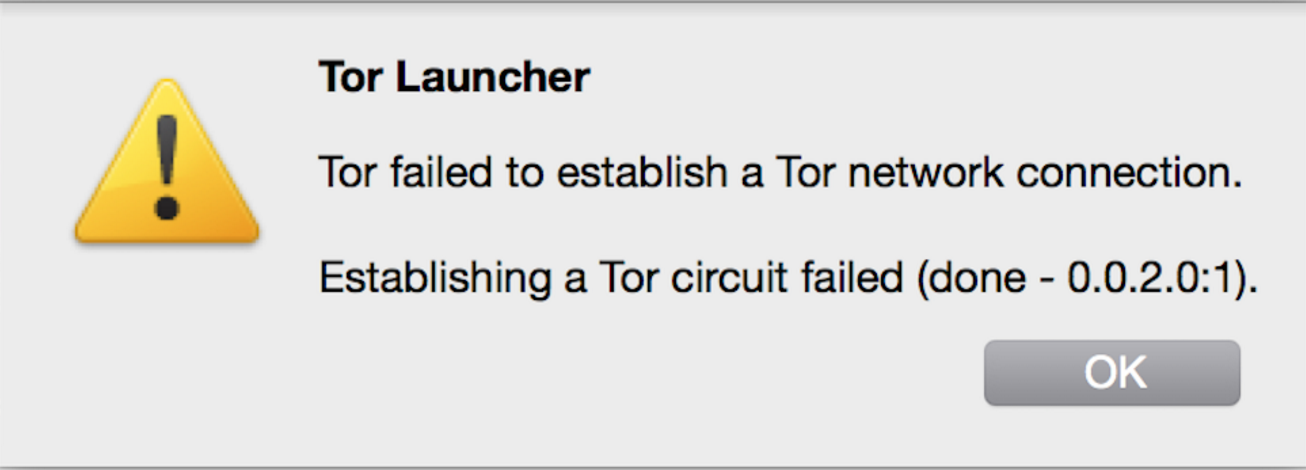
\includegraphics[width=0.5\textwidth]{error.png}
    \caption{An example of a technical error message which our participants did not understand.}
\label{fig:error}
\end{figure}
}

\section{Design Principles and Changes}
\label{sec:design} 

{\color {blue}
Introduction to security design principles. 

Security design principles: 
\begin{enumerate}
\item no user-dependent inputs 
\item no network-dependent inputs
\item minimal information leaks
\end{enumerate} 

%In principle, the process of configuring a proxy and bridge can be automated, but
%the interface eschews automatic configuration through network probing
%in favor of guided manual configuration to give users agency in configuring their connection. 
%Automatic configuration through network probing may put some users in certain regimes at risk. 
%A knowledgeable user can minimize their network trace and hide that they are connecting to Tor.
Justify why we kept the similar interface. Refer to appendix for alternative approaches. 

Introduction to usability design principles. 

Usability design principles: 
\begin{enumerate}
\item minimal user work
\item full user control  
\item targeted user feedback
\item build a mental model
\end{enumerate} 

Introduction to design changes.  \\

\noindent Changes made for minimal user work: 
\begin{itemize}
\item eliminated technical questions. Less questions to answer, less screens. 
\item auto-detection for proxies. A local scan of the operating system configuration does reveal information to network eavesdroppers and can detect if a proxy is used (if configured in other browsers). (We simulated the auto-detection by hard-coding the fact that a proxy was not required.)
\end{itemize} 

Changes made for full user control: 
\begin{itemize}
\item added intructions on what to try next on errors. The advice may be to try the connection again, to choose a different bridge, or to try a connection without a proxy. 
\item added advice for choosing connect versus configure. Before, the interface only informed users that the connect option worked some of the time, but did not specify why. We labeled the configure option as a manual option  specifically for users in heavily censored environments.
\item gave advice on choosing transports. We tell users to try a meek bridge if obfs3 does not work.
\end{itemize}

Changes made for feedback: 
\begin{itemize}
\item progress bar feedback fixed and network-accurate. We fixed the bug that caused the progress bar to not update on subsequent attempts. We switched the continuous progress bar to a discrete checkpoint-based progress indicator that shows the network components involved in connecting to the Tor network. 
\item minimized interface text. Whenever we could, we tried to shave text and keep it simple. 
\end{itemize}

Changes made to build a mental model:
\begin{itemize}
\item added system status visibility. We added a summary screen displays the current bridge and proxy settings
\item switched proxy and bridge configuration order. Network components are now configured in a topologically sequential order, resembling Fig.~\ref{fig:topology}.
\end{itemize}

Refer to figure with all deployed interface window (in previous section), refer to figure with all new interface windows (in caption, refer to appendix with advice text given on errors). Intorduce new/old labels. 
}

\section{Summative Usability Testing}
\label{sec:quantitative}

{\color {blue} 
short intro sentence.
}

\subsection{Recruitment}
{\color {red} 
We recruited 124 participants, about 20 for each
condition. We recruited half of our users from Craigslist, and half of our participants from 
the <redacted> %Xlab 
participant pool. Although <redacted> %Xlab 
participants are not limited to <redacted> %UC Berkeley 
students and staff,
a majority of the participants are from campus. For this reason, we chose to recruit 
half of our participants from Craigslist to ensure a diverse set of participants. 
The recruitment text vaguely suggests testing a piece of software, and does not require
that users provide information in advance (Appendix~\ref{quantitative-recruitment}). 
Out of our 124 participants, 59 were recruited from the <redacted> %Xlab 
pool and the other 65 were
recruited from Craigslist. Ages ranged from 18 to~68 years
($\mu = 28.9$, $\sigma = 12$). 56.8\% were male and 
84.8\% of our participants had at least a college education.
}

\subsection{Setup}
{\color {red} 
We ran our experiment at <redacted>.
%Xlab~\cite{xlab}, the Experimental Social Science Laboratory at the University of California, Berkeley. 
<redacted> %Xlab 
has 36 Windows~7 laptops, separated by cubicle walls. 
Though Tor Browser runs on other operating systems,
testing was only done on Windows, as a byproduct of using <redacted>. %Xlab. 

We augmented the interfaces with instrumentation 
to log every meaningful interaction
(button presses, menu selections, screen changes).
We wrote scripts to automatically set up the simulated censorship environment, install necessary software, 
start the video recording, and save the logs and videos.
We recorded the participants' computer screens
throughout the experiment to capture non-interface activity such as 
web searching and inspection of system networking settings.
}
\subsection{Procedure}
{\color {red} 
The one-hour, multi-participant procedure began when all participants sat at their
respective computers in <redacted>. %Xlab. 
Each computer was equipped with an instrumented old or new version
of Tor Browser, Chrome, Firefox, Internet Explorer,  Chrome, and VLC (for screen recording).
Each computer was assigned one of the six conditions in the beginning of the study. Participants
were assigned to a simulated censorship environment combination at random. 

A researcher informed the participants that they are in a
simulated censorship environment, instructed them to visit a sample blocked website on a 
non-Tor browser of their choice to illustrate the situation, and asked them to 
complete a worksheet that asks to visit one blocked website (Appendix~\ref{quantitative-script}). 
To mirror the qualitative study, we chose Wikipedia's featured article of the day 
as the blocked website to visit on their worksheet. 

After instructions, researchers maintained minimal interactions with the participants, 
only answering logistical questions.
The participants did not know the details of their censorship environment,
only that they are being censored. Participants had 40 minutes to configure Tor Browser to 
circumvent the simulated censorship and visit the blocked website. 

After users completed the browsing tasks, they took a short exit survey (Appendix~\ref{quantitative-exit-survey})
that collected their demographics. All users were instructed to sit until the end of the experiment,
regardless of when they had completed their task. After the 40 minutes, 
participants were officially informed that their time was up, and were given their payment of 
\$30 for their time. 
}

\subsection{Results} 
{\color {red} 
The possible interface version and environment combinations resulted in 6 experimental conditions. We recruited 124 participants to aim for about 20 participants per condition. We filtered participants who downloaded their own version of Tor Browser or did not sign the consent form, resulting in 114 participants. Table~\ref{table:participant-summary} summarizes the rate of success, time to success, and active time for our participants' by condition. 

%We refreshed a list of Tor relay IP addresses and added them
%to a firewall blacklist before each session.
%In the first study, we neglected to block the IP addresses
%of the Tor directory authorities, which are the first hosts
%a client contacts when initiating a non-bridge connection.
%New relays also appeared in the network on an hourly basis,
%which enabled a small number of participants to succeed with
%a direct connection when that configuration should have failed.
%We believe this is acceptable because 
%the qualitative user study was not used to quantify failures or successes, 
%but to explore possible problems.
%We fixed this problem in our quantitative user study by blocking the directory authorities.

%We blocked en.wikipedia.org, the target of the experiment,
%as well as other language-specific subdomains such as
%de.wikipedia.org and fr.wikipedia.org.
%We neglected, however, to block the Simple English Wikipedia
%at simple.wikipedia.org, which one participant found,
%thinking they had completed the task.
%% E2-OLD-X04-20160330-181928

%We discarded data on participants who chose to download their own version of Tor Browser online. 5 participants downloaded their own version without trying the provided one on their desktop, while others did so after feeling frustrated with the provided version. 

%Many waited for minutes at the progress screen, but never saw an error message. Error messages are intended to appear after a timeout. There were warnings, but those warnings went largely unnoticed by our participants. Across both versions of the interface, only one participant ever saw an error message. We tried to make error messages more instructive and understandable, since participants in our experiment did not encounter error messages, we cannot evaluate them. 

We summarize each participant's actions throughout the experiment in Fig.~\ref{fig:all-participant-edges}.
%and summarize where they spent their time in Appendix~\ref{all-participant-times}. 
Each row in Fig.~\ref{fig:all-participant-edges} corresponds to a participant. The bar represents a path through the interface, illustrating time spent on each screen, transitions between screens, how many attempts were made, and if they were eventually successful. 

\begin{figure*}
\centering
% This is a manually edited version of the automatically generated
% all-participant-edges graphic. It is edited to have better scale labels for
% the treatments.
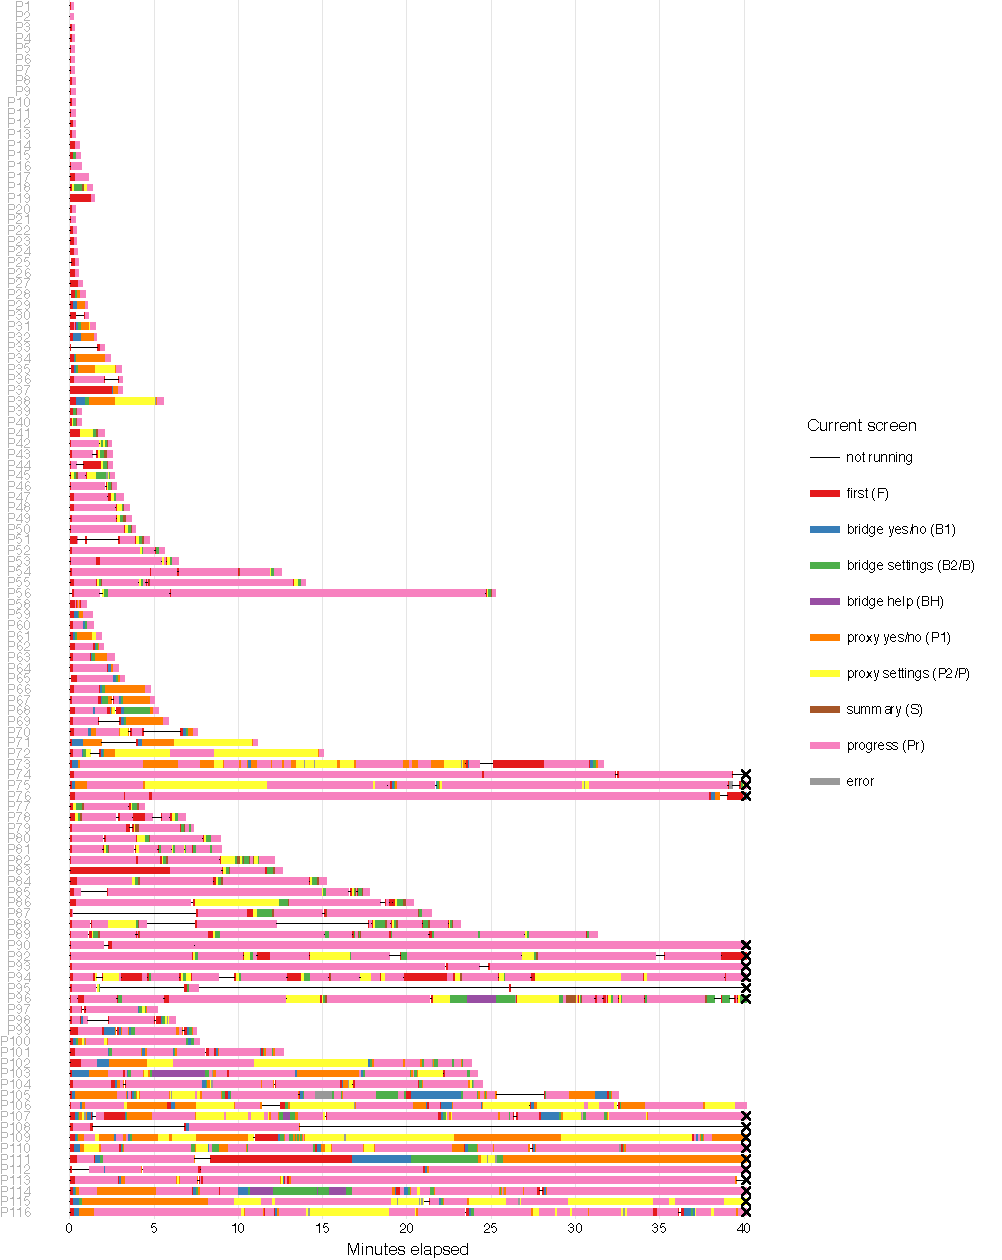
\includegraphics{all-participant-edges}
\caption{
Summary of participants' actions throughout the entire experiment.
Different colors indicate which screen was shown at each moment.
The ``not running'' times are those when Tor Launcher was closed;
i.e., a participant was doing something else
such as searching the web in another browser.
The overall length of the lines show the total time to completion,
except for those we cut off after approximately 40 minutes.
}
\label{fig:all-participant-edges}
\end{figure*}

\begin{table}
\centering
% Do not edit this file. Edit info.R instead.
\begin{tabular}{l r r r r r}
& \multicolumn{2}{r}{success rate} & \multicolumn{1}{r}{median time} & \multicolumn{1}{r}{median} \\
& \multicolumn{2}{r}{after 40 minutes} & \multicolumn{1}{r}{to success} & \multicolumn{1}{r}{active time} \\
\noalign{\hrule}
E1-NEW & 19/19 & 100\% & 0:20 & 0:06 \\
E1-OLD & 19/19 & 100\% & 1:01 & 0:24 \\
E2-NEW & 18/18 & 100\% & 3:22 & 0:40 \\
E2-OLD & 16/19 & 84\% & 5:00 & 2:04 \\
E3-NEW & 13/19 & 68\% & 20:25 & 1:56 \\
E3-OLD & 10/20 & 50\% & 40:08 & 9:06 \\
\end{tabular}

\caption{
A summary of participants' success in circumventing censorship
given their simulated censorship environment and version of Tor. Those who
failed to connect successfully were assigned the maximum time of 40:08.
}
\label{table:participant-summary}
\end{table}

\subsubsection{Rate of Success} 
49 of 56 (88\%) participants with the new interface successfully connected to Tor, while 45 of 58 (78\%) participants with the old interface did. Due to the limited number of participants, this difference is not large enough to rule out the possibility of random chance being the cause for the difference. Appendix~\ref{stat-tests} details the methodology for the statistical tests used in this paper. 

%\begin{figure}[t]
%\centering
%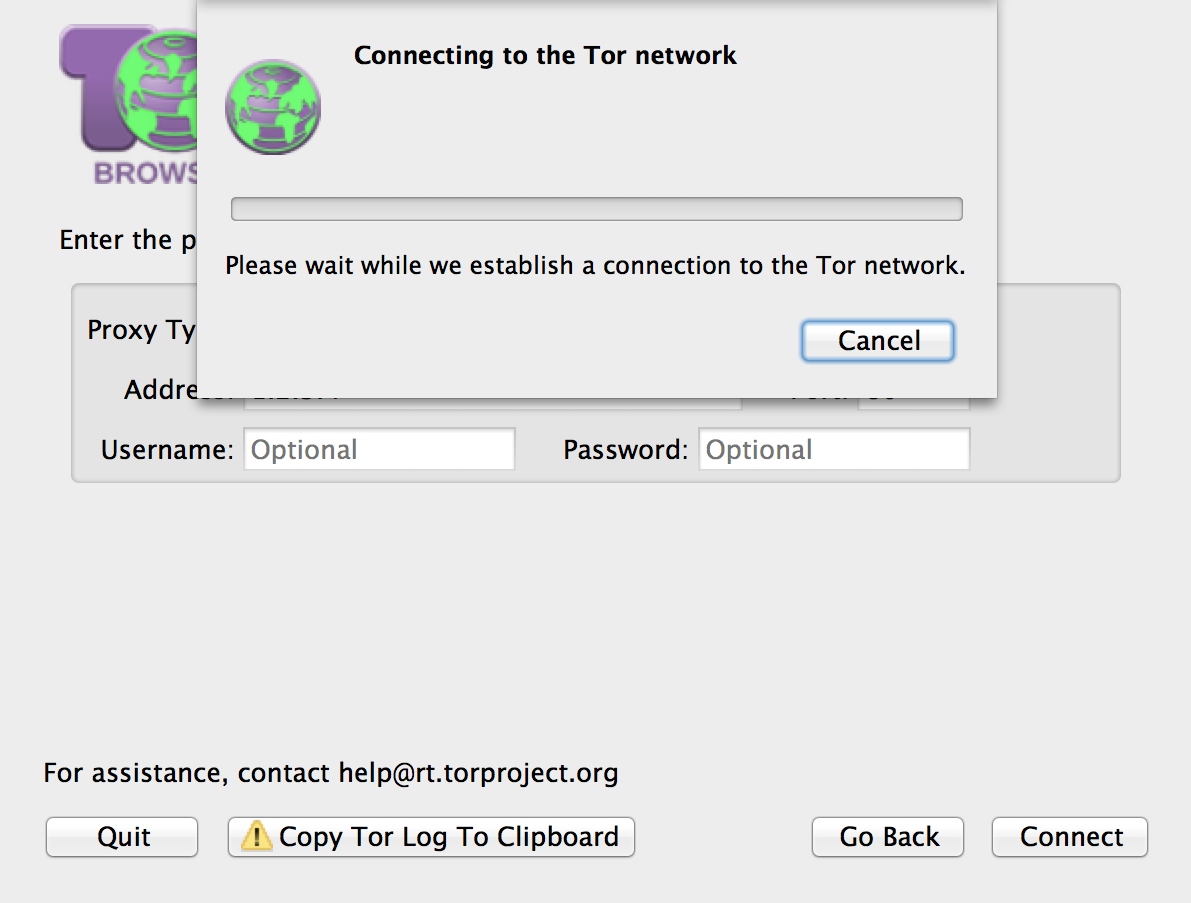
\includegraphics[width=.5\textwidth]{warning.png}
%\caption{
%A screenshot of the interface with the ``Copy Tor Log to Clipboard'' button, 
%which appears silently and does not interrupt the progress bar. 
%This warning was generated by entering in syntactically correct but invalid proxy settings,
%a mistake that prevents users from ever connecting to the Tor network. 
%Users are never directly notified of this error through an error message or a timeout message.
%Our participants made this error during our experiments, along with others that they were not notified about. 
%}
%\label{fig:warning}
%\end{figure}

%\begin{figure}[t]
%\centering
%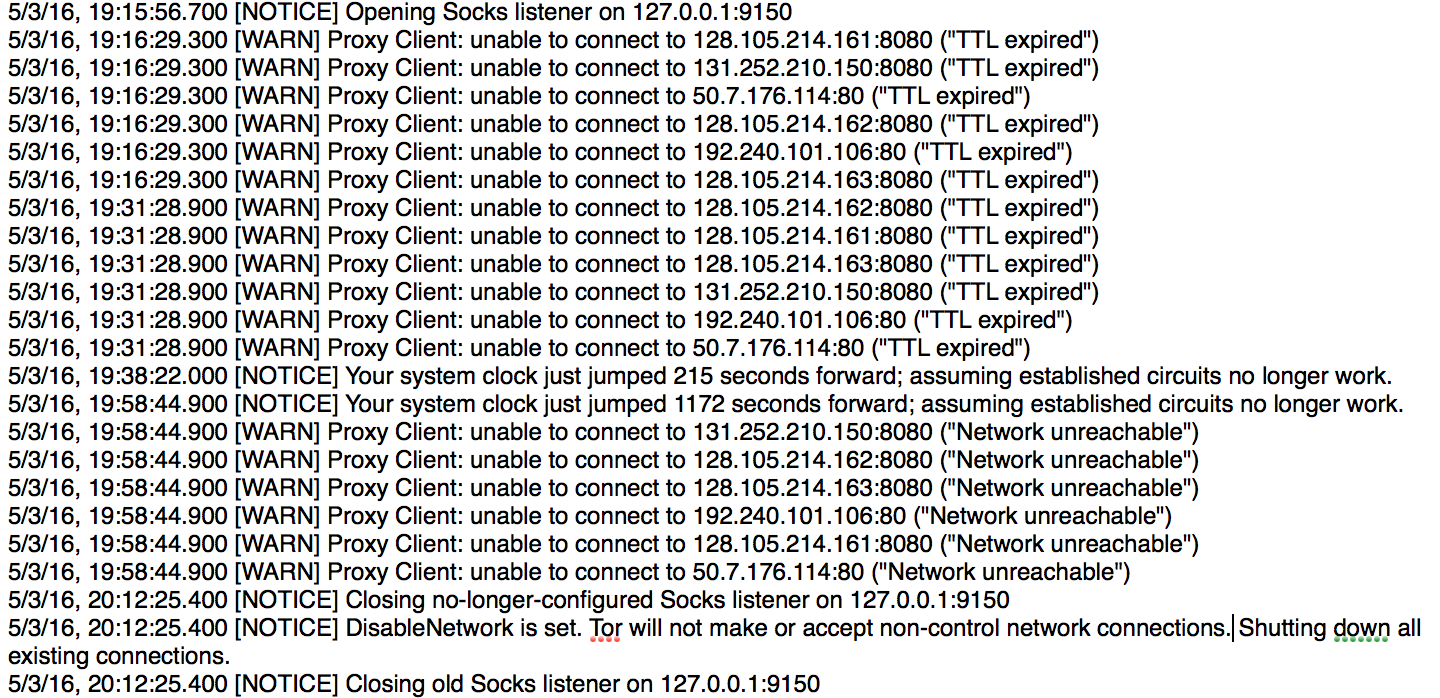
\includegraphics[width=.5\textwidth]{log-messages.png}
%\caption{
%The last 24 of 45 log lines that users receive after clicking clicking the ``Copy Tor Log to Clipboard'' button. 
%These log lines were the result of entering in syntactically correct but invalid proxy settings,
%a mistake that prevents users from ever connecting to the Tor network. Understanding the Tor logs require
%technical expertise from the user to understand the logs, diagnose the problem, and formulate next steps.
%}
%\label{fig:warning_log}
%\end{figure}

%We believe that the added advice on what to try next on error messages would have improved the rate of success. However, only 1 of 116 participants saw an error during the experiment. The old interface warned users on some mistakes (i.e. entering in a syntactically correct but invalid proxy settings) rather than displaying an error message. When a user receives a warning, a button that says ``Copy Tor Log to Clipboard'' silently appears at the bottom of the interface (Figure~\ref{fig:warning}). To see the log messages, users must click on the button, open up a text editor, and paste the log messages. The log messages require the user to understand the log, diagnose the problem, and formulate next steps (Figure~\ref{fig:warning_log}).

%The addition of a summary screen did cause behavioral changes (13\% of participants saw their current settings, then went back and adjusted them), but this behavioral change did not have a statistically significant impact on success rates. 

We added preemptive advice to the bridge configuration screen to first try an obfs3 bridge and then a meek bridge, but we suspect that most participants did not benefit from this advice since participants did not think to adjust their bridge settings upon failure. Of the 75 participants that failed to connect on the first attempt, 15 participants with the new interface and 13 participants with the old interface went back to the bridge screen and chose another hard-coded bridge. 10 of 15 in the new interface chose a meek bridge as their next bridge whereas 5 of 13 in the old interface chose meek as their next bridge, but we cannot claim choosing meek bridges is a direct result of our advice.

Table~\ref{tab:attempts-bridge-proxy} shows the configuration settings of the first successful connection in each environment and interface combination.We only consider the first successful connection since many of our curious participants tried many different settings to investigate if they will work, even after they had completed the task. Recall E1 does not require users to configure a bridge, E2 requires users to configure any bridge, and E3 requires users to configure a meek or custom bridge. Note that only four of the hard-coded bridges were used to connect successfully for the first attempt were the recommended bridge and the required bridges to succeed in E3.

Our participants did not optionally configure a bridge in E1 or configure a non-recommended bridge in E2. This suggests that users will not configure optional components or deviate from the recommended settings unless necessary. If the intent of the recommendation is to get as many users as possible to use the recommended bridge, this is a positive result. If the intent of the recommendation is to give pointers when users are stuck but allow the users to make their own bridge choices to diversify active transports, this is a negative result. 

Only two participants chose to configure a custom bridge. Both of these participants sent an incorrectly formatted request to the automatic bridge responder, which did not reply with custom bridges as a result. These two participants failed to connect to the Tor network. 

\begin{table}
\centering
% Do not edit this file. Edit attempts.R instead.
\begin{tabular}{r c c c c c c}
& \rotatebox{90}{E1-NEW} & \rotatebox{90}{E1-OLD} & \rotatebox{90}{E2-NEW} & \rotatebox{90}{E2-OLD} & \rotatebox{90}{E3-NEW} & \rotatebox{90}{E3-OLD} \\
no bridge, no proxy & 17 & 13 &  &  &  &  \\
obfs3, no proxy & 2 & 6 & 18 & 16 &  &  \\
meek-amazon, no proxy &  &  &  &  & 7 & 4 \\
meek-google, no proxy &  &  &  &  & 5 & 4 \\
meek-azure, no proxy &  &  &  &  & 1 & 1 \\
no bridge, 3rd-party proxy &  &  &  &  &  & 1 \\
DNF (did not finish) &  &  &  & 3 & 6 & 10 \\
\end{tabular}

\caption{
Bridge--proxy combinations that led to the first successful bootstrap
in each environment and interface.
Most E1 participants used a direct connection,
but a few tried a built-in obfs3 bridge.
All the E2 participants who succeeded,
did so with obfs3 (the recommended bridge type)---none tried
a different bridge before obfs3.
All of the successful E3 participants but one
used one of the meek bridges.
The remaining E3 participant succeeded in an unexpected way:
by searching the web for an open proxy and configuring it
as the proxy setting.
}
\label{tab:attempts-bridge-proxy}
\end{table}

% Is this the right place for this? 
% GENERAL STUFF; SHORTEN THIS A LOT
{\color {red} 
Additional stuff we found out through a combination of log processing (i.e. configuration settings on attempts) and video observation (i.e. watching what they searched for online).

How people succeeded. Straightforward. 

How people failed-- 17\% (19 of 114) of participants were not able to successfully connect to Tor. 63\% (72 of 114) of first attempts to connect failed and (363 of 458) of total attempts to connect failed. \\ 

\begin{description}
\item {\bfseries Some people won't try other options (6/19).} P73, P75, P89, P91, P106, P110 tried a direct connection. When that failed, they tried the same option, over and over, no matter how many times they failed. It was common to restart the interface, check Internet settings, and wait between subsequent attempts.

\item {\bfseries Recommendations work, but one and done (5/19).} P90, P93, P108, P111, P114, who were in E3, did not know what to do next after a direct connection and a default obfs3 bridge connection. They often tried those configurations again or gave up. 

\item {\bfseries People don't know what their problem is (5/19).} P74, P92, P105, P107, P113 assumed that they needed a proxy. They spent their time trying to configure a proxy, usually without trying other bridges. 

\item {\bfseries Bridges auto-responder is hard to use (2/19).} P94, P109, who were in E3, emailed the bridges auto-responder to get custom bridges. However, they formatted the message incorrectly and thus failed to get a response (Appendix~\ref{custom}).
\end{description}
} 

\subsubsection{Time to Success} 
Time to success is defined as the time until the first successful connection to Tor. Non-finishing participants are assigned the maximum experiment time of 40:08.  Our changes to the interface had a significant impact in reducing the time participants took to successfully connect to Tor (Mann--Whitney $Z = -1.84$, $p = 0.0328$, $r= 0.172$; see Appendix~\ref{stat-tests}). The simulated censorship environment also had an impact; the more difficult the censorship environment, the longer participants took to configure their connection (Kruskal--Wallis $\chi^2 = 80.5$, $\mbox{df} = 2$, $p < 10^{-15}$). 
Table~\ref{table:participant-summary} shows the median active times and Figure~\ref{fig:time_to_success_clamped} shows their distribution.

\begin{figure}[t]
\centering
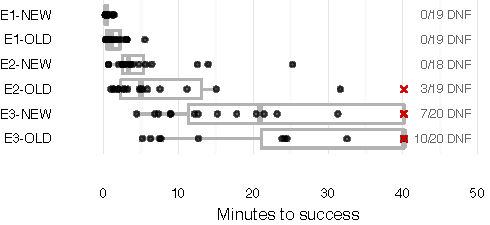
\includegraphics{time_to_success_clamped}
\caption{
Time to first success, by censorship environment and interface.
The dots show the raw completion times,
while the boxplots show the medians and interquartile ranges.
The ``DNF'' figures at the right show the number of participants 
who did not finish in the time allotted.
Here, non-finishing participants are assigned the maximum time of 40:08.
}
\label{fig:time_to_success_clamped}
\end{figure}

In our experiment, participants had 40 minutes to circumvent censorship. Fig.~\ref{fig:time_to_success_ecdf} shows the cumulative success rates over time. In practice, faster time to completion would mean more users will succeed, since users will give up after a while. Users in the wild will likely not be motivated to spend 40 minutes trying to configure Tor. If users were only willing to put in a minute or so of their time, users in intermediate and heavily censored environments would be unable to connect. Even if users were willing to dedicate 10 minutes to configuring their connection, most users in heavily censored environments would be unable to connect. Ideally, users should be able to connect to Tor within a few minutes, regardless of their censorship environment. We propose ideas on how to achieve this in section~\ref{recommendations}. 

\begin{figure}[t]
\centering
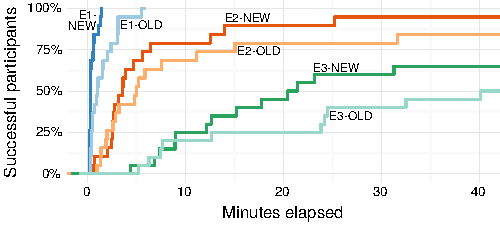
\includegraphics{time_to_success_ecdf}
../experiment/processing/time_to_success_ecdf.tex
\caption{
Cumulative success rates over time, by censorship environment and interface.
We stopped participants after 40 minutes. Here, those who did not finish were assigned
an arbitrarily high number greater than 40 minutes for the purposes of plotting. 
For example, every E1-NEW participant finished within 90 seconds,
but only 58\% of E1-OLD had finished by that time. Within 10 minutes, most
participants in E2 had finished, along with a minority of E3 participants. 
}
\label{fig:time_to_success_ecdf}
\end{figure}

\subsubsection{Active Time to Success} 
The overall time was largely dominated by the time spent waiting to connect to Tor, rather than actively configuring the interface. With correct configurations, the bootstrap process can take up to two minutes.  With incorrect configurations, a lack of error messages on the progress screen caused some users to wait indefinitely.  Logs show that participants spent 58\% of their overall time at the progress screen. Table ~\ref{table:median_time} shows the median percentage of time spent on each screen. 

\begin{table}[t]
\centering
\begin{tabular}{l r r r r}
& First & Proxy & Bridge & Progress \\
\noalign{\hrule}
E1-NEW & 28\% & 0\% & 0\% & 60\% \\
E1-OLD & 30\% & 0\% & 0\% & 29\% \\
E2-NEW & 6\% & 5\% & 6\% & 78\% \\
E2-OLD & 7\% & 18\% & 8\% & 45\% \\
E3-NEW & 3\% & 5\% & 5\% & 77\% \\
E3-OLD & 2\% & 12\% & 6\% & 64\% \\
\end{tabular}

\caption{The median percent of time spent on each screen, which is not
necessarily the median absolute time spent on that screen. 
This percentage is computed independently for each screen; that is, a participant who spent the median percent 
of time on one screen may not be the same participant who spent the median percent
of time on other screens. Note that the time spent on the progress bar dominates the 
time spent in the interface.} 
\label{table:median_time}
\end{table}

\begin{figure}[t]
\centering
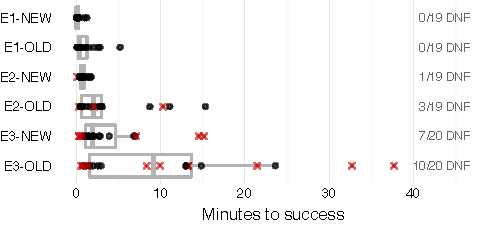
\includegraphics{time_to_success_active_clamped}
\caption{
Active time, by censorship environment and interface.
The dots show the raw active configuration times,
while the boxplots show the medians and interquartile ranges.
Here, non-finishing participants' active time was computed by
subtracting the amount of time spent on the progress screen from the 
the maximum time of 40:08.
}
\label{fig:time_to_success_active_clamped}
\end{figure}

Perhaps a more meaningful measurement is the amount of time participants actively configured their connection (Figure~\ref{fig:time_to_success_active_clamped}). We define active time as the time that participants spent interacting with the interface, excluding the time waiting for the connection to bootstrap. Active time for unsuccessful participants were calculated by subtracting the amount of time spent on the progress screen from the maximum experiment time, 40 minutes. This is an approximation, since some participants searched for help on the web after exiting the interface or on the progress screen. 

We performed a one-tailed Mann--Whitney test to compare the amount of active configuration time between participants who used the new interface and the participants who used the old interface. Our changes to the interface reduced the time participants spent configuring the interface (Mann--Whitney $Z = -3.28$, $p = 0.000516$, $r = 0.307$).  Table~\ref{table:participant-summary} shows the median active times and Figure~\ref{fig:time_to_success_active_clamped} shows their distribution.
%for color red
}

\section{Recommendations}
\label{recommendations}
We believe that adopting our design will help save users time when connecting to Tor. But we do not claim how much and in what way each change impacted our participants, since we did not test them independently. Some of our changes may have little or negative effects, but may be masked by other changes with positive effects. We also recognize that there may be equivalent or more impactful changes that may be made in place of ours. 

We hope that our inspection, design, and evaluation evaluation process provided valuable insight for potential changes. We do not recommend our specific design changes, but offer some advice and accompanying suggestions: \\

\begin{itemize}
\item {\bfseries Use less words.} While a thorough explanation isn't always possible with brevity, users are more likely to read the text if it is short.
\item {\bfseries Minimize work.} Ask users to perform tasks only when necessary. Hide less frequently used options or components. Redirect users to the relevant pages (i.e. redirect to the bridge screen the bridge fails).  
\item {\bfseries Give advice.} Guide users toward connecting directly unless they need a bridge or proxy, help them decide between transports, and discourage them from configuring optional components. 
\item {\bfseries Add system visibility.} Rather than requiring users to remember their bridge and proxy configuraitons, summarize their choices. The progress bar should reflect the current state of the connection.
\item {\bfseries Provide feedback.} In addition to displaying the error message, tell users what to try next when they encounter that error. 
\end{itemize}

We should consider alternative approaches of bootstrapping a connection to Tor. We recommend leveraging automation, user-dependent inputs, or network-dependent inputs for a solution that will help more users succed in a shorter amount of time. We start this discussion by sharing some of our own ideas in appendix~\ref{alternatives}. 

\section{Limitations}
\label{sec:limitations}
We did not study international users, or the configuration interface in languages other than English. All of our participants were from the United States and instructed to interact with the English version of Tor Browser.

Participants in a laboratory setting may alter their due to their awareness of being observed~\cite{mccarney2007hawthorne}. We are aware that our participants were likely motivated differently compared to real users. We believe that participants were likely overmotivated to connect to Tor because they were being observed and recieving a monetary reward. If true, this makes our results are a conservative estimate of the current problems. 

Since the configuration interfaces in simulated environments, we cannot claim how difficult it would be for a user to connect to Tor in a certain country or how much our redesigned interface would help those users.  

Our experiment did not directly test more advanced tasks. Our simulated environments did not require users to configuring a proxy or to get a custom bridge. From observing of user attempts to configure proxies and get custom bridges, we suspect users generally struggle with these tasks but cannot quantify how or why they do. 

We only tested interface on Windows machines, which were the machines available at <redacted>. %Xlab.
The configuration interface leverages the native operating system's styling and elements, making the configuration interface on Windows look slightly different from the OSx or Linux equivalent. Additionally, we acknowledge that participants' unfamilarity with Windows may have affected our experiment, but we believe that this affected all testing conditions equally.  

\section{Related Work}
\label{sec:related} 

{\color {red} 
There have been three published user studies on Tor. Clark et~al.~\cite{clark2007usability} examined various deployment
options for Tor Browser, such as Vidalia, Privoxy, Torbutton, and FoxyProxy, and found that none had satisfactory from a usability. Fabian et~al.~\cite{fabian2010privately} show that Tor's added
latency~\cite{dingledine2009performance} causes users
to be frustrated, cancel requests, and prevents user adoption. 
Norcie et~al.~\cite{norcie2012eliminating} found found that 
64\% of users are unable to continue with installation or browsing at least once due to difficulties.

We do not know of any published usability evaluations of
Tor Browser since the release of the 3.5 series in 2013, which introduced radical UI changes~\cite{torbrowser-35}.
The most recent effort is an unpublished pilot study by Lee and Fifield~\cite{uxsprint} 
that tested the downloading, installation, and browsing tasks in Tor Browser.  This study uncovered a number of issues~\cite{uxsprint2015-tickets},
some of which influenced changes in Tor Browser version~4.5 and later.

Previous user studies have considered the whole browsing experience,
without focusing on specific features in isolation.
Our study focuses on 
the browser's configuration interface, which guides users through setting up components required to circumvent censorship. 
%for color red
}

\section{Conclusion} 
\label{sec:conclusion}

{\color {blue}
We conducted a series of experiments to improve the Tor Browser 5.0.3 configuration interface. A couple sentences to summarize the whole thing. Echo roadmap in intro, but make it summary-like. 

%proof that user testing is important and general advice to for more research on Tor
Tor doesn't collect any information or perform AB testing, so this type of user research is especially important. to set it up, get users, computers, consent, and instrumented versions of the software. Research can be exploratory (ask users what they want), observational (look at what they do), or testing a hypothesis (verify changes). We encourage the use of simulated censorship environments as a tool for user testing censorship circumvention software. Not only do simulated environments avoid rerouting traffic through a censoring country's networks, their reproducibility and stability are ideal for experiments. 
}

%\section {Resources} 
%For additional details, such as the censorship simulation code, interview transcriptions, and logs of participant interactions, we refer you to the project repository: \\
%
%\noindent \url{https://github.com/lindanlee/circumvention-ux-tor}
%
%\section {Acknowledgments}
% Rowilma del Castillo of Xlab supported out experiment by assisting with testing, offering recruitment services, and allowing experiments after-hours. Nima Fatemi, Isabela Bagueros, Georg Koppen, and the Tor UX team have provided me with valuable feedback along the way. 

\bibliographystyle{abbrv}
\bibliography{pets2017-paper}

\appendix
\section{Alternative Approaches} 
\label{alternatives}
{\color {blue}
Our goal was to deploy impactful, tested changes the Tor configuration interface. In fact, Tor version~4.5 incorporated textual and navigational changes based on our redesigned interface. Throughout our experiments, we collaborated with Tor developers and focused on discovering changes that could be deployed right away. For this reason, we assumed that the configuration process will remain a manual process that requires user inputs, as it is currently deployed. However, we list some alternative approaches that seem worth exploring. \\

%remember: 	no user inputs, no network inputs, minimize info leaks
%and:		minimal user work, full user control 

\begin{description}
\item{\bfseries Automate the configuration.} The most efficient way to connect as many users to the Tor network is to automatically configure their connection on start. A naive automation is to try configurations that would most likely work, in order (i.e. a direct connection, then an obfs3 connection without a proxy, then an meek bridge connection with out a proxy). This leaks to network eavesdroppers that the user is connecting to the Tor network. We do not know how much risk is associated with this approach. 
\item {\bfseries automate after the first failure.} The network leak happened. But then this automation would be pretty fingerprintable behavior. 
\item{\bfseries Ask about the risk.} An alternative to naive automation is to offer manual configuration to those that want to be more cautious and automatically configuring a connection for who are not at risk. The complication with this approach is that users may not be qualified to answer if they are at risk or may not trust Tor with this information. 
\item{\bfseries Ask if users know what to do.} Another alternative to naive automation is to offer manual configuration to those that know how to configure their connection and to automate the process for users who do not know how to configure their connection. This may prevent the most mistakes, but does not account for the users' risk associated with using Tor. 
\item{\bfseries Suggest configurations.} A way to help users without any automation or questions is to give users information about what would work in their country. The first page of the configuration interface can show a list of countries with a corresponding recommended configuration. This approach does not require users to answer about their risk, technical ability, or location. However, it does require that the user trust the given advice and to correctly configure their settings based on this advice. 
\item{\bfseries Assign configurations.} This is a smart way to automate connections to the Tor network. Upon start, the interface detects proxy settings and uses them, if any. Then, all users connect to bridges that will always work (such as meek bridges), which assign them a guard relay based on their location, effectively assigning bridges for the user. 
\end{description}

We believe that automation, asking about risk, and identifying struggling users could enable significant improvements to the configuration process. 
%for color red
}

\section{Qualitative User Study Recruitment Posting} 
\label{qualitative-recruitment}
We are recruiting participants for an in-person research study at <redacted>. %the University of California, Berkeley. 
You will need to come in to our lab and perform tasks on a computer for an hour or less. You will be compensated \$30 for participating. 
No special knowledge and no technical experience is required. If you are interested, fill out the survey at \textit{<survey link>}. 

\section{Qualitative User Study Prescreening Survey} 
\label{qualitative-prescreening}
We are recruiting participants for an in-person research study at the <redacted>. %University of California, Berkeley. 
You will need to come in to our lab and perform tasks on a computer for an hour or less. You will be compensated \$30 for participating. No special knowledge and no technical experience is required.\\

\begin{enumerate}
\item{Please select when you are available. We will assign you an hour experiment time slot during one of those times.}
\item{I am able to provide my own transportation to the <redacted> %University of California, Berkeley 
campus.}
\item{Thank you for your interest! Please provide an email address where we can contact you to share more logistical details.}
\item{we are looking for a very small number of participants, so unfortunately, we may not be able to accommodate everyone who applies. Would you like us to let you know about future opportunities?}
\item{What is your gender?}
\item{What is your age?}
\item{Please select your highest completed (or current) level of education.}
\item{What is your occupation?} 
\item{Do you speak any languages other than English fluently?}
\item{If you have a personal computer, what kind do you use?}
\item{Which of the following terms have you heard of? \textit{<answer choices: a checkboxlist of the the following terms: malware, proxy services, phishing, SSL, X.511 certificates, Tor>}}
\item{How often do you use the following software or features? \textit{<answer choices: a grid of radio buttons. Software/features (rows): HTTPS on web pages, proxies or other censorship circumvention tools, virtual private networks (VPN), file or whole-disk encryption, anonymity systems (e.g., Tor), email encryption (e.g., PGP), chat or instant messaging encryption, voice communication encryption. Frequency (columns): never, less than once a month, a few times a month, several times a week, daily.>}}
\end{enumerate}
Thank you for filling out this form. You are now done!

\section{Qualitative User Study Introduction Script} 
\label{qualitative-script} 
Imagine you live in an oppressive country that censors part of the Internet. We have simulated this in the laboratory by blocking certain websites and services.  The purpose of this experiment is to evaluate the use of Tor browser, which is a browser that can circumvent censorship and let you visit blocked websites. Currently, torproject is blocked (you can check this by going to torproject.org on a standard browser, like Firefox, Chrome, or Internet Explorer). 

To circumvent censorship successfully, you will need to set up Tor browser correctly and use it to get to Wikipedia. If you are able to reach the website, then you know that you have successfully circumvented censorship. Fill out the question on the worksheet. This isn't intended to be hard, just write what you see. We want to just check you saw the website. 

Before you start, do you have any questions about what you are asked to do? 

\section{Participant Worksheet Text} 
\label{participant-worksheet}
Imagine you live in an oppressive country that censors part of the Internet. We have simulated this in the laboratory by blocking certain websites and services. The purpose of this experiment is to evaluate the use of Tor browser, which is a browser that can circumvent censorship and let you visit blocked websites. For instance, www.torproject.org is blocked. Check this by going to the site on a standard browser, like Firefox, Chrome, or Internet Explorer. It will fail to load, when you can visit other sites.

To complete this worksheet, you will need to set up Tor browser (on your desktop) correctly and use it to get to blocked site. If you can visit wikipedia, then you know that you have successfully circumvented censorship.

\section{Post-Experiment Standard Interview Questions}
\label{interview-questions}
We asked our participants these questions after they were given time to configure Tor Browser. \\

\begin{enumerate}
\item{Can you talk us through what you did along with what you were thinking at the time?}
\item{What was most challenging part of connecting?}
\item{Were there any unfamiliar terms?}
\item{How did you decide which options to choose?}
\item{What did you think about using Tor?}
\item{What is one change you would recommend?} 
\item{Did you need any additional information?} 
\end{enumerate}  

In addition to these questions, we asked our participants about specific questions based on their observation, usually regarding a specific choice in action, a particular screen they seemed stuck on, and any errors they encountered during the configuration process. 

\section{Quantitative User Recruitment Posting}
\label{quantitative-recruitment}
We are recruiting up to 40 participants for a user study at <redacted>. %UC Berkeley. 
The experiment will involve basic Internet browsing tasks. You are not eligible if you have participated in our previous sessions.\\

\indent Payment: \$30 Amazon gift card\\
\indent Duration: 1 hour \\
\indent Where: <redacted> \\ %Xlab at Hearst Memorial Gymnasium\\

\textit{<list of sessions>}\\

To be eligible, you must be an adult (18 or older). This is to comply with university policies on research. 

If you are interested: 1. Email <redacted> %lnl@berkeley.edu 
with the sessions you are able to attend. We will confirm your participation and assign you a session. 
2. Come to <redacted> %Xlab 
at the appointed time for the experiment.

\section{Quantitative User Study Introduction Script} 
\label{quantitative-script} 
Imagine you live in an oppressive country that censors part of the Internet. We have simulated this in the laboratory by blocking certain websites and services.  The purpose of this experiment is to evaluate the use of Tor browser, which is a browser that can circumvent censorship and let you visit blocked websites. Currently, torproject is blocked (you can check this by going to torproject.org on a standard browser, like Firefox, Chrome, or Internet Explorer). 

To circumvent censorship successfully, you will need to set up Tor browser correctly and use it to get to Wikipedia. Tor is already installed for you. On the desktop, you should see a globe icon that says ``Start Tor Browser.'' If you are able to reach the website, then you know that you have successfully circumvented censorship. Fill out the question on the worksheet. This isn't intended to be hard, just write what you see. We want to just check you saw the website. 

Afterward, we ask you to take a short survey to collect some information about you. The link is also on your worksheet.
We will give you time to complete this task. If you finish early, we ask that you sit at your desk until the remainder of the hour. Since we are recording your screen, we ask that you don't do anything personal afterward, like checking your email.

Before you start, do you have any questions about what you are asked to do? 

\section{Quantitative User Study Exit Survey} 
\label{quantitative-exit-survey}
We'd like to know more about you.  All of your answers will be stored separately from any identifying information in order to protect your confidentiality.

This survey is part of a research project being conducted by the <redacted>. %University of California, Berkeley. 
If you have any questions about your rights or treatment as a research participant in this study, please contact the <redacted>'s %University of California at Berkeley's 
Committee for Protection of Human Subjects at 510-642-7461, or email 
<redacted>. %subjects@berkeley.edu. 
If you agree to participate, please click Next below.\\

\begin{enumerate}
\item{What is your participant ID? (This can be found on the sticker on the left hand corner of the desk you are currently sitting at.)}
\item{What is your gender?}
\item{What is your age?}
\item{Please select your highest completed (or current) level of education}.
\item{What is your current occupation?}  
\end{enumerate}

Thank you for participating in our experiment. You are now done! Please sit at your desk for the remainder of the experiment. Our researchers will formally announce the end of the experiment. 

\section{Statistical Tests} 
\label{stat-tests}
{\color {red} 
From our measurements, we observe that participants with the new interface 
have a higher rate of success, succeed in less time, and configure their interface in less time. 
We do not find that the increased rate of success with the new interface or the decreased time to success with the new interface significant. That is, random chance can account for the difference. 
We do find the the decreased active configuration time to be significant. 
We describe the methodology for the statistical tests used in this paper to determine the impact of the interface on success rate, time to success, and active time. 

%success rate and version
Each participant had a boolean variable indicating a successful connection to Tor. Rates of success were calculated by dividing the number of participants who succeeded the condition over the total number of participants in the condition. This gave us six rates of success. E1-NEW, E2-NEW, and E3-NEW rates of success were compared against E1-OLD, E2-OLD, and E3-OLD.  We used a Pearson's Chi-squared test to test the significance of success rates. The difference between success rates of participants with the new interface and participants with the old interface was not significant ($X^2 = 0.0126$, $df = 2$, $p = 0.994$).

%time to success and version
Time to success was measured as the time from the participants started the Tor launcher interface to the first successful bootstrap to the Tor network. This measurement was 1) non-normal and heavily right-tailed since participants were less and less likely to succeed as time went on and 2) right-censored at 40 minutes, the maximum time of the experiment. Because of the right-tailed nature of the data, we used a one-tailed Mann--Whitney test. Because the Mann--Whitney test does not account for right-censored data, we assigned the participants who did not succeed the maximum time of 40 minutes for the purpose of this test. We find the difference of times to success between participants with the new interface and participants with the old interface to be significant ($ Z = -1.84$, $p = 0.0328$, $r= 0.172$). 

%active time and version
Active configuration time was measured as the time the participants spent in the Tor launcher interface, except for the time spent the progress screen. For our participants who did not succeed to connect to Tor, subtracted the time spent on the progress screen from the maximum experiment time of 40 minutes. This measurement was also 1) non-normal and heavily right tailed and 2) impacted by right-censored measurement of time to success. Because of the right-tailed nature of the data, we used a one-tailed Mann--Whitney test. We find the difference of active configuration times between participants with the new interface and participants with the old interface to be significant ($Z = -3.28$, $p = 0.000516$, $r = 0.307$).
%for color red
}

\end{document}
